\chapter{Treats}

\section{Fermina's Ginger Snaps\index{treats!gingersnaps}}

\textit{This is a super-yummy cookie recipe sent in from
Fermina.  She tells us that she always doubles this 
recipe when making a batch. Maybe the
increased amounts of ingredients help the taste factor.  Either that or we're
just gluttons.  Here's the recipe.} 
\begin{ingredients}
3/4 cup of shortening \\ 
1 cup sugar \\ 
1/4 cup light molasses \\ 
1 slightly beaten egg \\ 
2 cups flour \\ 
1/4 tsp.  salt \\ 
1 tsp.  cinammon \\ 
2 tsp. soda \\ 
1 tsp.  clove \\ 
1/2 tsp.  ginger
\end{ingredients} 
Cream shortening and sugar, add molasses
and egg.  Mix all dry ingredients.  Stir dry ingredients into creamed mixture. 
Spoon into balls. Added step for yumminess:  \textit{Drop spoonfulls into sugar
before putting on baking sheet}.  One spray of water before baking.  Bake
350$^{\circ}$ for 8 to 10 minutes.  The cookies should be split in the middle
when finished.

\section{Betsy's Chocolate Chip Poundcake\index{treats!chocolate chip pound
cake}}

\textit{This is the famous Betsy Cordova's Chocolate Chip
Cake. When she e-mailed this to use she sent a request for many treat
recipes.  What we tell her we tell all.  Send us a recipe and you get a book.  
This serves however many you feel like depending on your hunger.}
\begin{ingredients}
3 cups sugar \\ 
2 sticks butter \\ 
6 eggs \\
3 cups flour  \\
1 carton heavy whipping cream (small size) \\ 
2 Tbsp.  vanilla \\ 
1/2 bag mini chocolate chips 
\end{ingredients}
Cream butter and sugar, add 2 eggs and 1 cup flour and beat.  Add 2 eggs and 1
cup flour and beat. Add 2 eggs and 1 cup flour and beat.  Mix in vanilla and
whipping cream and add chocolate chips.

Bake in greased and floured bundt pan at 350$^{\circ}$ degrees for 60 to 75
minutes (depending on the temperature of your oven).

\vspace{2\baselineskip}
\centerline{
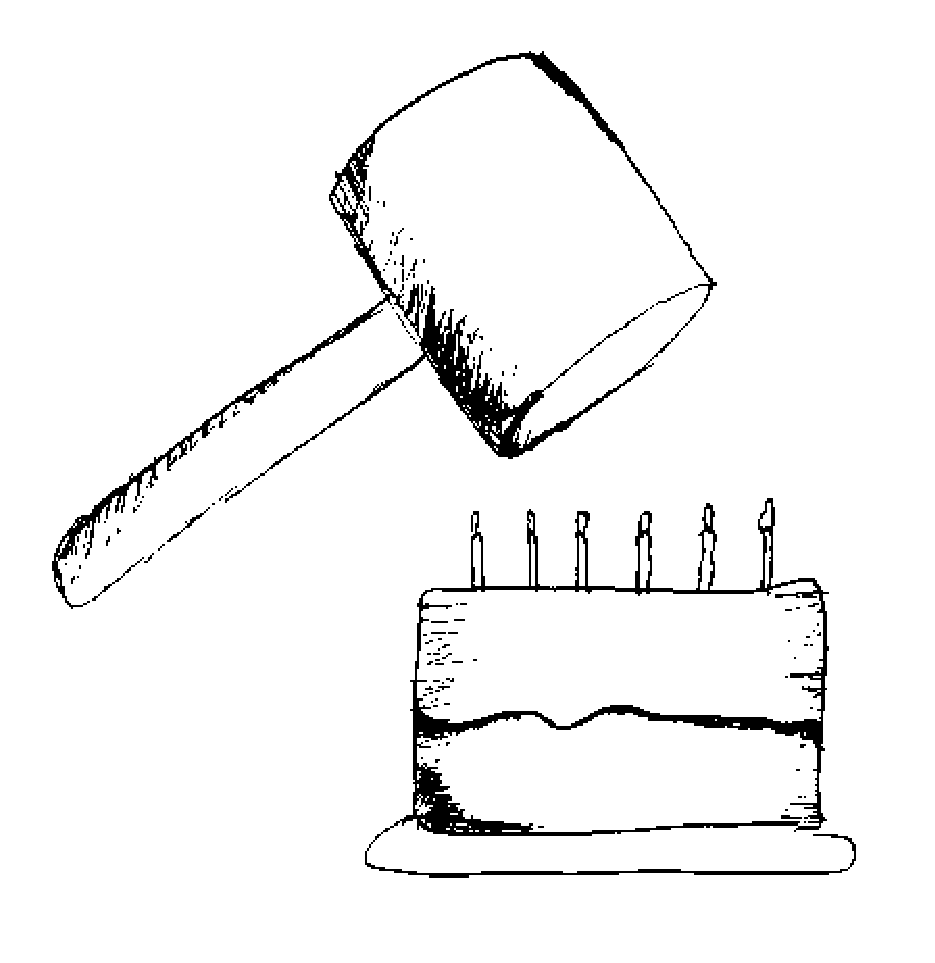
\includegraphics[scale=.5,clip]{pound.ps}}
\vspace{2\baselineskip}

\section{Amy's Cheesecake\index{treats!cheesecake}}

\textit{This is a holiday favorite at the Evans/Gormley households by
 Amelia Gormley.}
\begin{ingredients}
1 box Graham Craker Crumbs \\
1/2 cup sugar \\
2 Tbsp.  flour \\
1/4 tsp.  salt \\
1 pound cream cheese \\
1 tsp.  vanilla extract \\
4 eggs \\
1 cup heavy cream
\end{ingredients}
The topping ingredients are:
\begin{ingredients}
2 cups sour cream \\
3 Tbsp.  sugar \\
1 tsp.  vanilla
\end{ingredients}
Follow the directions on the Graham Craker Box for the crust.  
Use a 9$''$ spring form pan.  Press crumb mixture into the bottom 
and sides of the pan.

%\begin{wrapfigure}{r}{1.5in}
%\centerpicture 3.19in by 2.75in (pie scaled 300)
%\end{wrapfigure}
Let cream cheese soften at room temperature (or use microwave).  Mix sugar,
flour, and salt.  Add dry ingredients to cream cheese.  Cream together with low
speed beater or by hand.  Seperate eggs, save the whites in a clean bowl.  Add
yolks to cream cheese mixture and beat until smooth.  Add vanilla.  Stir in
cream.  Beat egg whites until stiff.  Fold into cream cheese mixture.  Pour on
top of crumbs.  Bake at \oven{350} for 1 hour.  Let cool.  Mix topping
ingredients.  Pour topping onto cheesecake and bake at \oven{500} for 10
minutes.  Serve with cherry, blueberry, etc. etc. toppings.

\section{Pineapple Upside-down Cake\index{treats!pineapple upside-down cake}}

\textit{Kate: On his/her birthday most kids I knew asked for chocolate cake, or
ice-cream cake,  or even cheesecake if  sophisticated. But not Tom.
Tom always begged for this somewhat unusual birthday cake. Luckily, Fermina
Evans has a great recipe for it!
Tom: I begged for it because it's delicious. Any kid would agree.}
\begin{ingredients}
1/2 cup butter \\
1/2 cup packed brown sugar \\
1 large can pineapple slices in syrup \\
1 small jar maraschino cherries
1\ 1/2 cup non packed flour (softasilk flour recommended) \\
1 cup sugar \\
2 tsp. baking powder \\
1/2 tsp. lt \\
1/3 cup soft shortening \\
2/3 cup milk \\
1 tsp. vanilla \\
1 large egg
\end{ingredients}
Melt butter with brown sugar in 9" baking pan (Fermina adds 1 Tbsp. Karo syrup
here) Arrange pineapple slices on top of syrup and place cherries in pineapple
centers or wherever they look nice. 

In mixing bowl, stir flour, sugar, baking powder and salt. Add shortening,
milk, and vanilla. Beat 2 minutes at medium speed with electric mixer. Add egg
and beat two more minutes. Pour batter over fruit. Bake at \oven{350} for
40-50 minutes. Immediately turn upside
down on serving dish (if you don't, sugar will crystallize to pan and you will
have a mess). 

\section{Chocolate Mint Brownies\index{treats!chocolate mint brownies}}

\textit{Kate: Blah blah blah chocolate blah.  Tom:  These are yummy!  My mom
makes them}.
\begin{ingredients}
1 cup sugar\\
1/2 cup butter or margarine\\
4 eggs, beaten\\
1 cup flour\\
1/2 tsp. lt\\
1 can \corp{Hershey's Chocolate Syrup} (16 oz.)\\
1 tsp. vanilla
\end{ingredients}
Mix together above ingredients and put in a greased $9''\times 13''$ pan. 
Bake at \oven{350} for 30 minutes.

The middle layer ingredients are:
\begin{ingredients}
2 cups pwedered sugar\\
1/2 cup butter or margarine\\
2 Tbsp \corp{Creme de Menthe} (preferably the green kind
\end{ingredients}
Mix and spread over cooled cake.

The glaze ingredients are:
\begin{ingredients}
1 cup chocolate chips\\
6 Tbsp butter
\end{ingredients}
Let the cake cool slightly and spread over brownies.  Chill and cut into
squares.

\section{Gooey Butter Cake\index{treats!gooey butter cake}}

\textit{A recipe from Fermi's friend Pam L.}
\begin{ingredients}
1 pkg. yellow cake mix\\
1/2 cup melted butter\\
1 egg
\end{ingredients}
The topping ingredients are:
\begin{ingredients}
8 oz. cream cheese (1 pkg.)\\
2 eggs\\
1 box powdered sugar
\end{ingredients}
Preheat oven to \oven{350}.  Mix together cake ingredients.  Pat into
$9''\times 13''$ pan.  Beat topping ingredients together for three minutes.
Pour over cake mix.  Bake for forty minutes.  Do not overbake. Top should be 
set, but not dry.

\section{Chocolate Surprise\index{treats!chocolate surprise}}

\textit{Fermi's chocolate \& angel food cake.  George's birthday favorite.}
\begin{ingredients}
32 large marshmellows\\
1/3 cup water\\
1/4 tsp. lt\\
6 oz.\ semi-sweet chocolate chips\\
heavy whipping cream and sugar\\
1/4 tsp. vanilla
\end{ingredients}
\begin{wrapfigure}{l}{2.0in}
\centerline{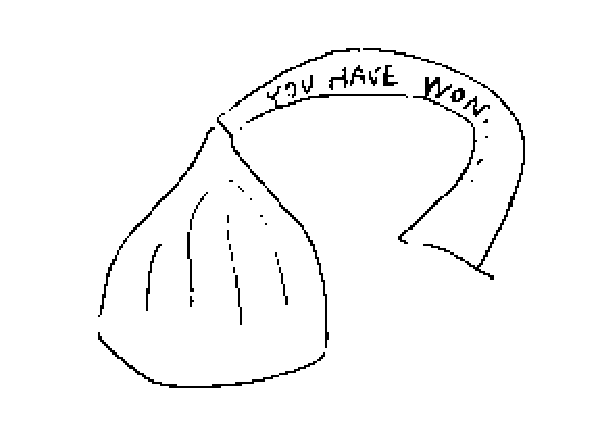
\includegraphics[width=1.8in,clip]{kiss.ps}}
\end{wrapfigure}
In sauce pan melt marshmellows, water, and salt.  Add chocolate bits.  Stir
until melted.  Let cool.

Whip 1 cup whipping cream.  Pour chocolate over cream and fold together.

Take a store brought or home make angel food cake.  Cut off entire top 1$''$
layer.  WIth spoon dig a tunnel in remaining cake.  Fill with chocolate
surprise.  Replace top layer.

Sprinkle cake with powdered sugar or frost with whipped cream (1 cup heavy
cream beaten with 1 Tbsp. sugar until stiff).  

\section{Tiramisu\index{treats!tiramisu}}

\textit{Mimi Horne brings us this delicious treat from an
Italophile Brazilian Yale Art History Professor friend, Ester da Costa Meyer.
Those in less gastro-enlightened regions might need to replace the mascarpone
with cream cheese and cream, and the Marsala with perhaps port or sherry. }
\begin{ingredients}
2-3 pkgs (about 24-30) lady fingers (boudoirs) \\
3 cups mascarpone (or part creme fraiche, part carre frais mushed together)\\
3 egg yolks \\
1/3 cup sugar \\
2 cups strong coffee \\
1/2 cup or more Marsala wine \\
1/2 cup cocoa
\end{ingredients}
Prepare coffee and mix with Marsala. One at a time, dip lady fingers in mixture
briefly, then lay them in a row in an approx. $10''\times 18''\times 2 1/2''$
deep serving dish.
Cut some to fit the remaining space in dish so that the bottom is
completely covered. Mix sugar, egg yolks and mascarpone/cream. Spread
about half the mixture over the first layer of cookies to cover completely.
Dip more lady fingers in coffee/Marsala and lay them over cream to form the
next layer; cover remaining cream mixture. Dust the top thoroughly with cocoa;
chill overnight or for several hours before serving. More cocoa may be added
before serving. The texture can be made lighter by beating the egg whites and
folding them into the mascarpone mixture, which also increases the amount.
Serves 6-8.

\section{Tortelettes\index{treats!Tortelettes}}

\textit{Another Nonnie/Grandpatty and Joy of Cooking original. Niepold kids
remember Christmas at Lee St. when they eat Tortelettes and California dates
stuffed with Georgia Pecans and rolled in confectioners' sugar.}
\begin{ingredients}
1 grated lemon rind\\
1 cup sugar\\
3/4 cup butter\\
2 egg yolks \\
1/2 cup bread flour \\
1 cup blanched and shredded almonds or pecan pieces \\
1/3 cup sugar \\
1 tsp. cinnamon\\
1/4 tsp. nutmeg\\
1/8 tsp. salt\\
1 egg white\\
1 Tbsp water
\end{ingredients}
Preheat oven to \oven{375}. Grate lemon into sugar. Cream sugar with butter and
beat in the egg yolks one at a time. Add flour gradually to make a stiff
dough. Pinch off about a teaspoonful of dough at a time. Roll it into a ball
and flatten on cookie sheet until very thin. Prepare nuts and combine with
next 4 ingredients (spices). Beat the egg white and water together slightly.
Brush the cakes with the egg white mixture, then sprinkle nut/spice mixture
and bake until light brown.  

\section{Lime Cream Pie\index{treats!Lime Cream Pie}}

\textit{Kate got this recipe from Edie, a receptionist at Bryn Mawr College
with southern cooking blood. 
It's very easy and delicious, especially after a rich
meal. It's cool, refreshing, and slides right down.}
\begin{ingredients}
1 Graham Cracker Pie Crust\\
3 egg yolks\\
2 2/3 cups sweetened condensed milk (2 cans)\\
1 cup plus 2 Tbsp lime juice (about 7 limes if you're squeezing)\\
2 tsp. grated lime zest\\
1 attractive lime
\end{ingredients}
Lightly whisk egg yolks in mixing bowl. Pour in
condensed milk and whisk until completely blended.  Add lime juice and zest and
whisk to blend. Gently pour filling into pie crust shell and smooth over top.
Refrigerate for at least 4 hours (don't skimp or it will be soup!). Slice
the attractive lime paper thin to garnish. I like to slice into
half-circles and create a pinwheel pattern around the center. 
